\documentclass[a4paper,11pt]{article}
\usepackage[T1]{fontenc}
\usepackage[utf8]{inputenc}
\usepackage{lmodern}
\usepackage{hyperref}
\usepackage{graphicx}
\usepackage{rotating}
\usepackage{listings}
\usepackage{color}

\title{AlphaBiscuit - Image Recognition of Letter Biscuits}
\author{Arash Rouhani}
%\affiliation{Chalmers University of Technology}
%\email{rarash@student.chalmers.se}

\date{May 30, 2011}

\begin{document}

\maketitle

\begin{abstract}
    Letter biscuits have been around for many decades, but digital image
analysis are only beginning to find applications in the real world.
Typing with letter biscuits is joyful for children, using image analysis
one could create electronic activities that involves these biscuits,
such activities could improve literacy among children. This paper take
a statistical approach to automatically classify alphabet biscuits,
applying known techniques from image analysis. Using the classifier, we
then create a word reader that extracts words from an image of letter
biscuits.
Result wise, the final classifier performs near-perfect in the cross-validation,
however it doesn't always identify all biscuits in a clean 'word-image'.

\end{abstract}

\section{Introduction}
The recognition of letter biscuits is similar to many other image recognition problems.
Image recognition being well developed already, only little new research have been made for this project.
Rather, a way to combine existing techniques will be presented.

In order to optimize our recognition method, some remarks should be made on the type of data we are working with.
To our favour, the biscuits are manufactured, and therefor all biscuits
of the same letter looks the same, both in shape and color.  On the
other hand the solid body form of biscuits can suppress distinguishable
characteristics. For example, the hole in the letter A is small, perhaps
unnoticeable, due to the overall thickness of the biscuits. Another
problem, when dealing with letter recognition in general is the multitude
of letters to identify from.

The identification process is a standard composition of image processing
concepts. Segmenting, collecting features and then classifying.
Initially we segment a picture to a black and white image containing
only the biscuits, we then collect features from the segmented image.
The classification is based on the features, we classify the unknown
biscuit by comparing its features to a set of known biscuits.  In case
of there being several biscuits in the image, a wordizer will organize
the letters and read out the word.

The segmentation process is well studied for \emph{general} objects, but the fact that the biscuits are of the same colors must be used.
One challenge is to develop our own segmentation method.
The method created for biscuit segmentation could also be used for other segmentation purposes where the data is having similar properties.

\section{Data collection}
Initially, a mobile camera was used to photograph all the images.
Later this was changed to use a much better camera with more organized photography.
The biscuits are laid on a blank white paper, so the whole background is white when photographing, this avoids to catch anything with similar colors as the biscuits on the image, as that would distract the segmentation.
There is no deliberate noise, the lightning is stabilized by the use of camera lightning and the camera was put stable on a tripod.
All the biscuits used are from the commercial brand named BRAGO BOKSTAVSKEX.
Figure \ref{fig:unprocessed} contains two typical unprocessed images from the data set.

\begin{figure}[]
\begin{center}
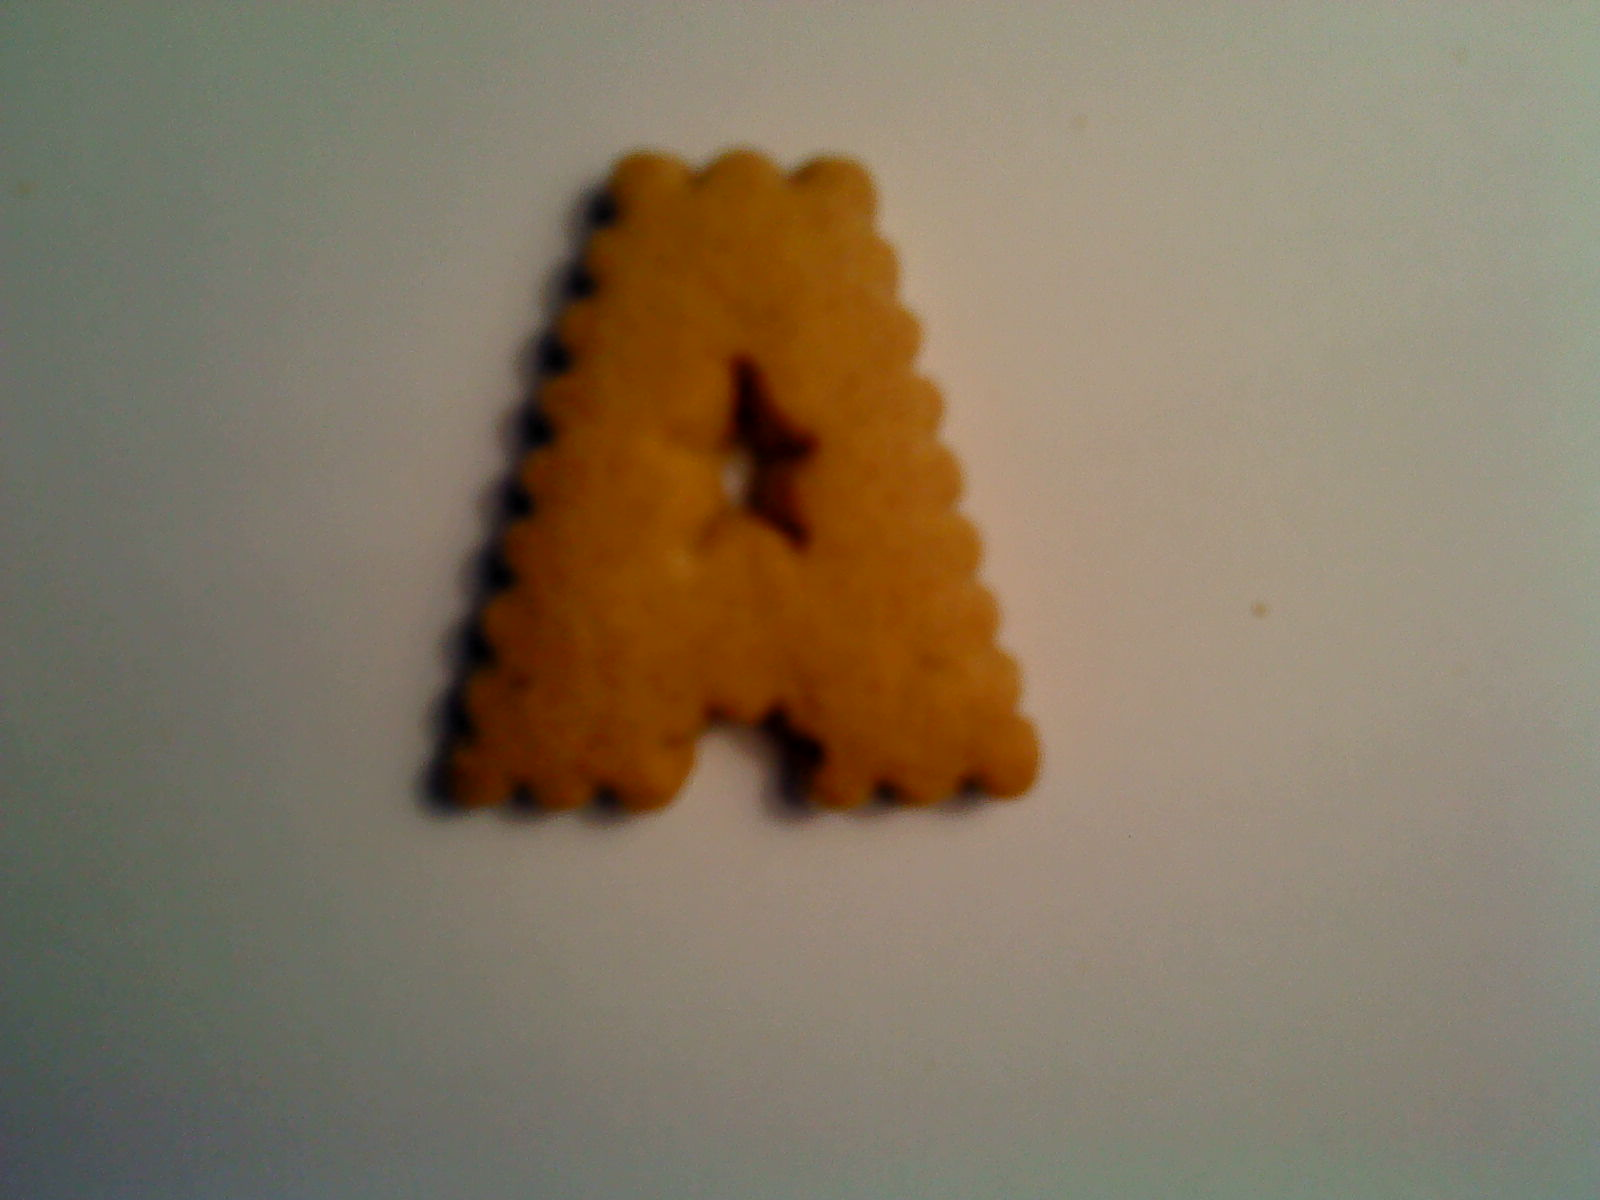
\includegraphics[width=40mm]{orig_a.JPG}
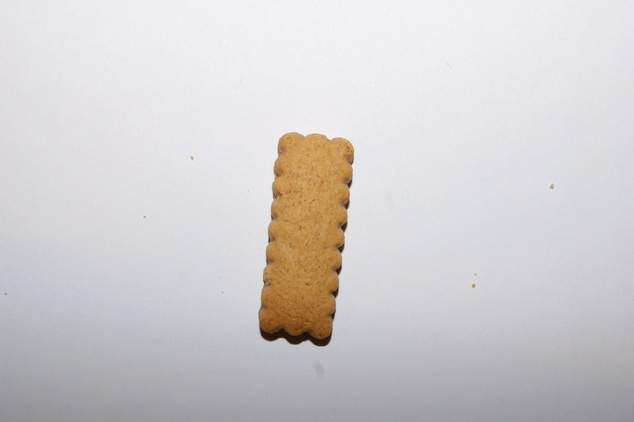
\includegraphics[width=40mm]{orig_i.JPG}
\end{center}
\caption{Two unprocessed images}
\label{fig:unprocessed}
\end{figure}

Among the biscuits, there are only capital letters present. A few letters are missing.
There are totally $177$ images of single biscuits that the classifier trained on.
Figure \ref{fig:alphabet} shows all the characters present in the data.

\begin{figure}[]
\begin{center}
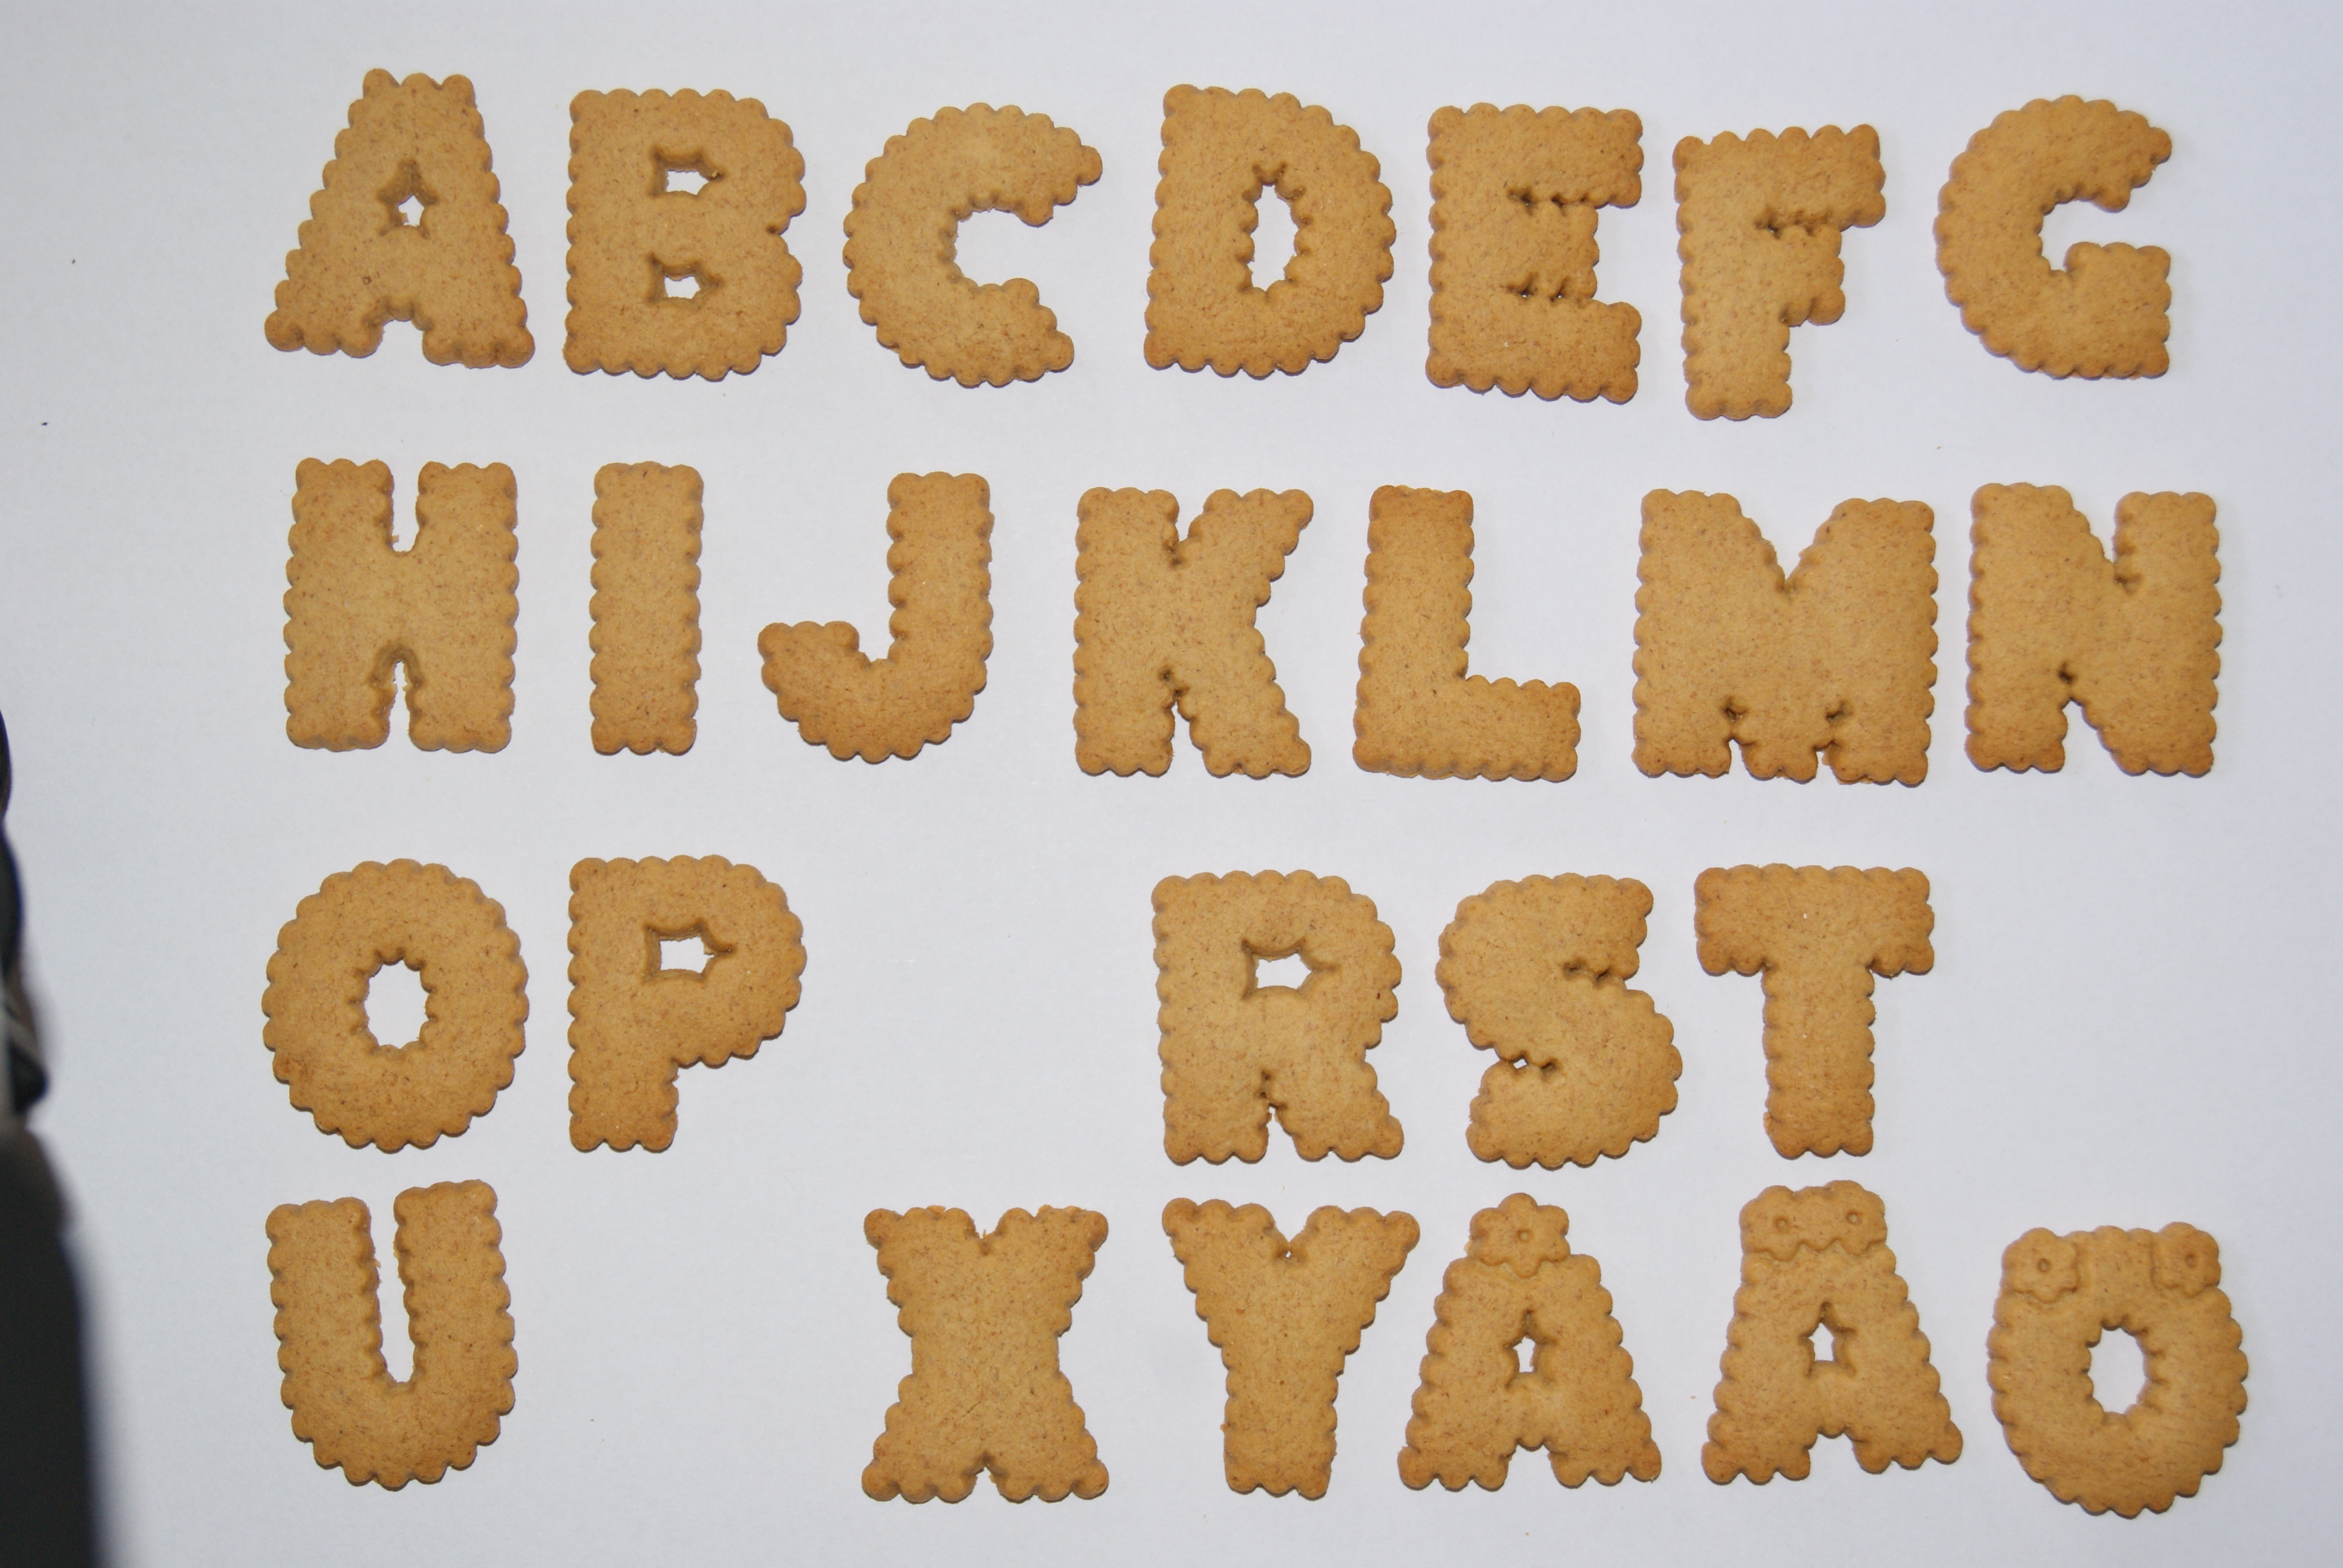
\includegraphics[width=140mm]{alphabet.JPG}
\end{center}
\caption{An image of all the character types present in the data set}
\label{fig:alphabet}
\end{figure}

\section{Segmentation}

When studying the biscuits as an \emph{object},
it's clear that the biscuits are only of one color,
but when studying \emph{images} of biscuits, 
the pixels corresponding to the biscuit varies in color because of different lightning.
As humans this don't bother us, we automatically segment objects apart.
In image analysis, segmenting means to decide which pixels are actually of interest to us.
There are many known segmentation methods available.
And they work differently good for different segmentation tasks.

We want a segmentation method that uses the fact that the biscuits are of the same color.
One sensible segmentation method is to define a set of the RGB-colors representing usable colors.
That means pixels are interesting only if its color is in the set.

In this project, we implemented our segmentation with the above mentioned ideas in mind.
Since it worked sufficiently well, we did not examine more possibilities. 
\emph{Thresholding} can quite easily implement the set idea in practice.

\subsection{Thresholding}
We threshold directly on the color image, treating each pixel individually. 
That means that we don't threshold on grey-scale images,
neither do we turn a color image into grey-scale as an intermediate step.

With expressivity over the three color channels, 
we can easily define a reasonable set of biscuit-colors.
For example, the biscuits are always more red than green, and always more green than blue.
With thresholding this property can be easily stated as $r>g>b$.
The exact mathematical thresholding used in our implementation is
$ r > 50 \wedge 30 < g < 200 \wedge b < 150 \wedge r > 1.2*g \wedge g > 1.2*b $.
Where $\wedge$ stands for logical conjunction. r, g and b stands for the red, green and blue component of the RGB-component, respectively.

The input images are also of a low JPG quality, meaning that adjacent pixels can vary more than they are supposed to.
To battle this, we also run a Gaussian filter on each color channel before thresholding.


\begin{figure}[]
\begin{center}

\includegraphics[width=40mm]{seg_a.png}

\includegraphics[width=40mm]{seg_i.png}
\end{center}
\caption{Two segmented images using thresholding}
\label{fig:segmented}
\end{figure}


\section{Features}
We use the following features:
\begin{itemize}
\item Major Axis Length
\item Solidity - Also called convexity
\item Momentum - An easily turnable (easy for a given mass) object has a high momentum, for example the letter I. Momentum is calculated by summing for each pixel it's distance from the center-weight. The momentum feature can be measured for different exponents on the distance for each pixel. We used three features of this kind with exponents 1,2 and 3.
\item Eccentricity
\item Perimetry
\item Number of holes - An \emph{A} has one hole, but a \emph{B} has two holes.
\end{itemize}
It should be noted that the feature Number of holes isn't fail proof,
since bad segmentation can create holes, or cover actual holes.
\subsection{Feature normalization}
The features presented above are incomparable to each other.
When MajorAxisLength have been normalized with respect to the area, 
it can be compared to another MajorAxisLength value, 
even though the zooming of the pictures are not the same. 
However, the feature MajorAxisLength is incomparable to features of a different type.

In the configuration in table \ref{tab:features}, it's clear that the Solidity reveals that the biscuits
are different, the MajorAxisLength are however not to different.
However, when naively comparing by subtraction, MajorAxisLength has a bigger difference.
To battle this behavior we use the \emph{linear scaling with unit variance} normalization, see equation \ref{eqn:univariance} (Aksoy and Haralick, 2000).

\begin{table}[h!b!p!]
\caption{Two features of two biscuits}
\begin{center}
    \begin{tabular}{ l | c | c | }
                    & Biscuit 1 & Biscuit 2 \\ \hline
    MajorAxisLength & 7.0       & 8.5       \\ \hline
    Solidity        & 0.11      & 0.9       \\ \hline
    \end{tabular}
\end{center}
\label{tab:features}
\end{table}

\begin{equation}
x_{new} = \frac{x - \mu}{\sigma}
\label{eqn:univariance}
\end{equation}

After this transformation, all features have a mean of $0$ and variance of $1$.
Now it's more sensible to compare two different features, or to take the euclidean distance between two biscuits (set of features).
\subsection{Feature selection}
With feature normalization taken in place, there is yet no weighting of the features,
perhaps a large difference in MajorAxisLength definitely tells two biscuits apart,
meanwhile a large difference in Solidity should be considered less significant.

We do partially address this problem by using \emph{binary} weights on the features, 
that is equivalent to simply not using some features.
This is helpful when a feature is having a negative impact on the overall classification.
We use the \emph{greedy backward elimination} method in our feature selection.
\section{Classifying unknown biscuits}
Classification, in our case, is to determine the letter of an unknown biscuit, given the features of manually classified biscuits.

We use the simple \emph{Nearest Neighbour} classifier, with distance defined as the euclidean distance.

\section{Wordizer}
If an image contains many letters, the letters are often representing words.
The wordizer is sweeping through the letters and makes one sentence with the letters by examining the positions of each letter.
If visually clear enough, the wordizer will put whitespace (spaces and newlines) in the sentence where appropriate.
\section{Results}
The result section will show the results of a cross-validation process, look at a failing example and end with a section about reading out a word image.
\subsection{Cross-validation}
Given the data described, using the classification methods mentioned, we ran the backwards-elimination process.
Starting with the features listed in the features section, table \ref{tab:backelim} shows what features
where eliminated and for what gain.
The CV-value is the ratio of correctly identified biscuits using cross validation over the total number of biscuits.


\begin{table}[h!b!p!]
\caption{Backwards elimination}
\begin{center}
    \begin{tabular}{ | l | c | c | }
    Feature         & Previous CV-value \\ \hline
    Solidity        & 97.18\%           \\ \hline
    Number of holes & 97.77\%           \\ \hline
    \end{tabular}
\end{center}
\label{tab:backelim}
\end{table}

So the final feature configuration became: Perimetry, Eccentricity and all three versions of momentum.
That configuration gave us a CV-value of $98.87\%$.
One missclassificatio can be seen in figure \ref{fig:misclas},
an E was misclassified for an K. The K have a distance of $0.331$,
and the closest correct character have a distance of $1.226$.
Their normalized features can be seen in \ref{tab:misclas},
it is $15$ candidates between the K and the closest E.

\begin{figure}[]
\begin{center}

\includegraphics[width=40mm]{original.png}

\includegraphics[width=40mm]{closest.png}

\includegraphics[width=40mm]{closest_correct.png}
\end{center}
\caption{An example of a misclassification. 
         The left image is the one we tried to classify. 
         The middle image is the closest neighbour.
         The right is the closest correct neighbour.}
\label{fig:misclas}
\end{figure}

\begin{table}[h!b!p!]
\caption{Normalized features of three biscuits in Figure \ref{fig:misclas}}
\begin{center}
    \begin{tabular}{  l | c | c | c | }
     Feature           & Left  & Middle & Right \\ \hline
     Eccentricity      &  0.55 & -0.01  &  0.56 \\ \hline
     Perimetry holes   &  0.87 &  0.91  & -0.24 \\ \hline
     Momentum degree 1 & -0.45 & -0.48  & -0.46 \\ \hline
     Momentum degree 2 & -0.35 & -0.30  & -0.36 \\ \hline
     Momentum degree 3 & -0.32 & -0.23  & -0.34 \\ \hline
    \end{tabular}
\end{center}
\label{tab:misclas}
\end{table}


Running the same procedure on a slightly reduced character-set without å, ä and ö,
the final feature configuration is Perimetry, Eccentricity, Solidity and momentum with exponent one.
That configuration yields a CV-value of exactly $100\%$. 

\subsection{Wordizing}
Wordizing the Image in figure \ref{fig:dreaming} gives the following output:

\texttt{ \\
dkxåhing \\
hxn äåx \\
uäunted \\
men \\
}

The same procedure with the reduced character-set yields the interpretation:

\texttt{ \\
dkeaming \\
hen are \\
uaunted \\
men \\
}

The newlines and spaces were automatically identified by the wordizer.
No other wordizing was performed.

\begin{figure}[]
\begin{center}
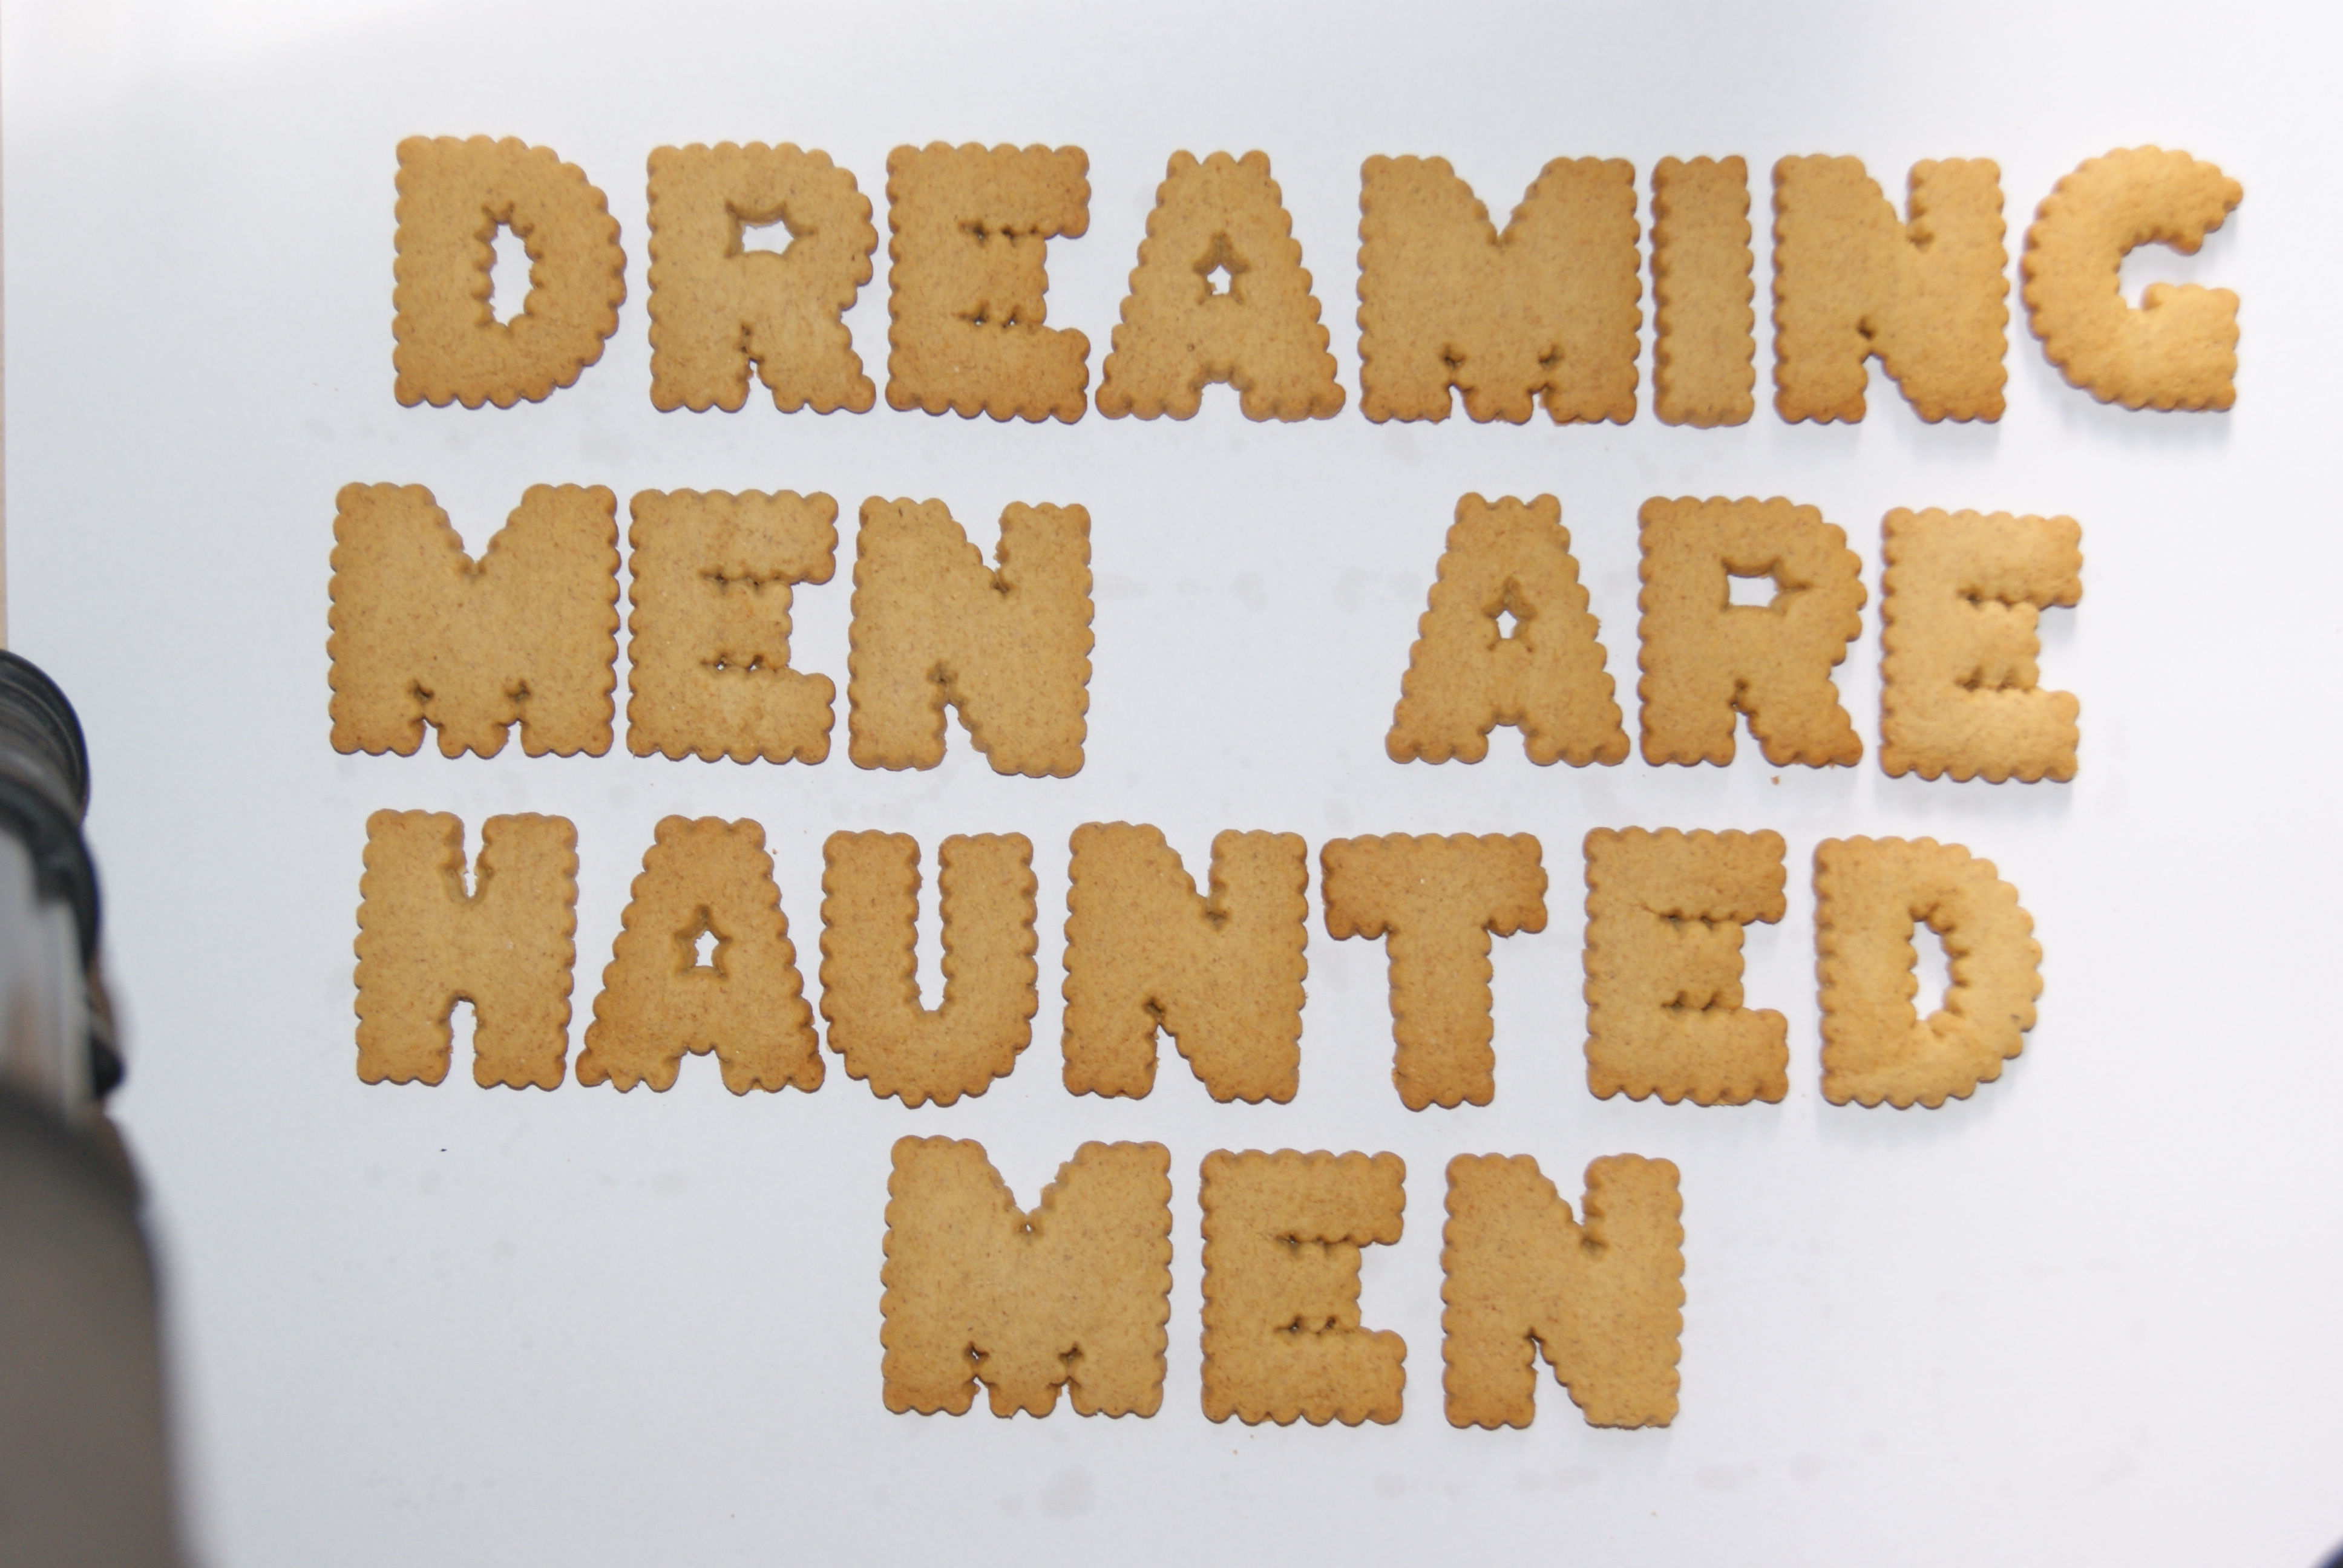
\includegraphics[width=140mm]{dreaming.JPG}
\end{center}
\caption{An image that can be wordized}
\label{fig:dreaming}
\end{figure}


\section{Discussion}

Even though overall simplicity, especially in classification, the cross-validation results are very good.
But on the other side, the input images are friendly to work with.
An undocumented experiment showed a CV-value of about 85\% with the old data-set 

The feature elimination shows a shaky behavior.
For the two data sets, that are very much alike,
two quite different set of features was suggested by backwards-elimination.
This might be due to that with the full data-set,
most of the effort by backwards-elimination was to minimize frequent a, å and ä clashes.
But with a data-set without such worries, the elimination focused on smaller details.

The result of the cross-validation where good, but the wordizing didn't perform as good.
It's however not reliable to state the condition of the project
based on one image. It would be interesting to try the wordizer on more examples.

The misclassification seen in Figure \ref{fig:misclas} is most likely
because of the bad segmentation at the bottom of the E.
At the same time, it's also obvious that some feature
should be able to clearly distinguish the E from the K.
Perhaps a feature that can detect the 'cracks' in the top and bottom
of the K would distinguish E from K.

\section{Conclusions}
The classifier performed outstanding in the cross-validation, 
but could not read out a word correctly, however word reading have not been
carefully measured in this report.

All features examined are rotation invariant, but the wordizer requires a normally angled view to assemble the words correctly.
The data worked on were very simple.
If a set of less clean images where to be used,
it would only be necessary to improve the segmentation part.

\section{Appendix}
All code, images and more is available at the project's \href{https://github.com/Tarrasch/AlphaBiscuit}{github page} .



\end{document}
